\documentclass[11pt,a4paper]{report}
\usepackage[textwidth=37em,vmargin=30mm]{geometry}
\usepackage{calc,xunicode,amsmath,amssymb,paralist,enumitem,tabu,booktabs,datetime2,xeCJK,xeCJKfntef,listings}
\usepackage{tocloft,fancyhdr,tcolorbox,xcolor,graphicx,eso-pic,xltxtra,xelatexemoji}

\newcommand{\envyear}[0]{2025}
\newcommand{\envdatestr}[0]{2025-04-03}
\newcommand{\envfinaldir}[0]{webdb/2025/20250403/final}

\usepackage[hidelinks]{hyperref}
\hypersetup{
    colorlinks=false,
    pdfpagemode=FullScreen,
    pdftitle={Web Digest - \envdatestr}
}

\setlength{\cftbeforechapskip}{10pt}
\renewcommand{\cftchapfont}{\rmfamily\bfseries\large\raggedright}
\setlength{\cftbeforesecskip}{2pt}
\renewcommand{\cftsecfont}{\sffamily\small\raggedright}

\setdefaultleftmargin{2em}{2em}{1em}{1em}{1em}{1em}

\usepackage{xeCJK,xeCJKfntef}
\xeCJKsetup{PunctStyle=plain,RubberPunctSkip=false,CJKglue=\strut\hskip 0pt plus 0.1em minus 0.05em,CJKecglue=\strut\hskip 0.22em plus 0.2em}
\XeTeXlinebreaklocale "zh"
\XeTeXlinebreakskip = 0pt


\setmainfont{Brygada 1918}
\setromanfont{Brygada 1918}
\setsansfont{IBM Plex Sans}
\setmonofont{JetBrains Mono NL}
\setCJKmainfont{Noto Serif CJK SC}
\setCJKromanfont{Noto Serif CJK SC}
\setCJKsansfont{Noto Sans CJK SC}
\setCJKmonofont{Noto Sans CJK SC}

\setlength{\parindent}{0pt}
\setlength{\parskip}{8pt}
\linespread{1.15}

\lstset{
	basicstyle=\ttfamily\footnotesize,
	numbersep=5pt,
	backgroundcolor=\color{black!5},
	showspaces=false,
	showstringspaces=false,
	showtabs=false,
	tabsize=2,
	captionpos=b,
	breaklines=true,
	breakatwhitespace=true,
	breakautoindent=true,
	linewidth=\textwidth
}






\newcommand{\coverpic}[2]{
    % argv: itemurl, authorname
    Cover photo by #2~~(\href{#1}{#1})
}
\newcommand{\makeheader}[0]{
    \begin{titlepage}
        % \newgeometry{hmargin=15mm,tmargin=21mm,bmargin=12mm}
        \begin{center}
            
            \rmfamily\scshape
            \fontspec{BaskervilleF}
            \fontspec{Old Standard}
            \fontsize{59pt}{70pt}\selectfont
            WEB\hfill DIGEST
            
            \vfill
            % \vskip 30pt
            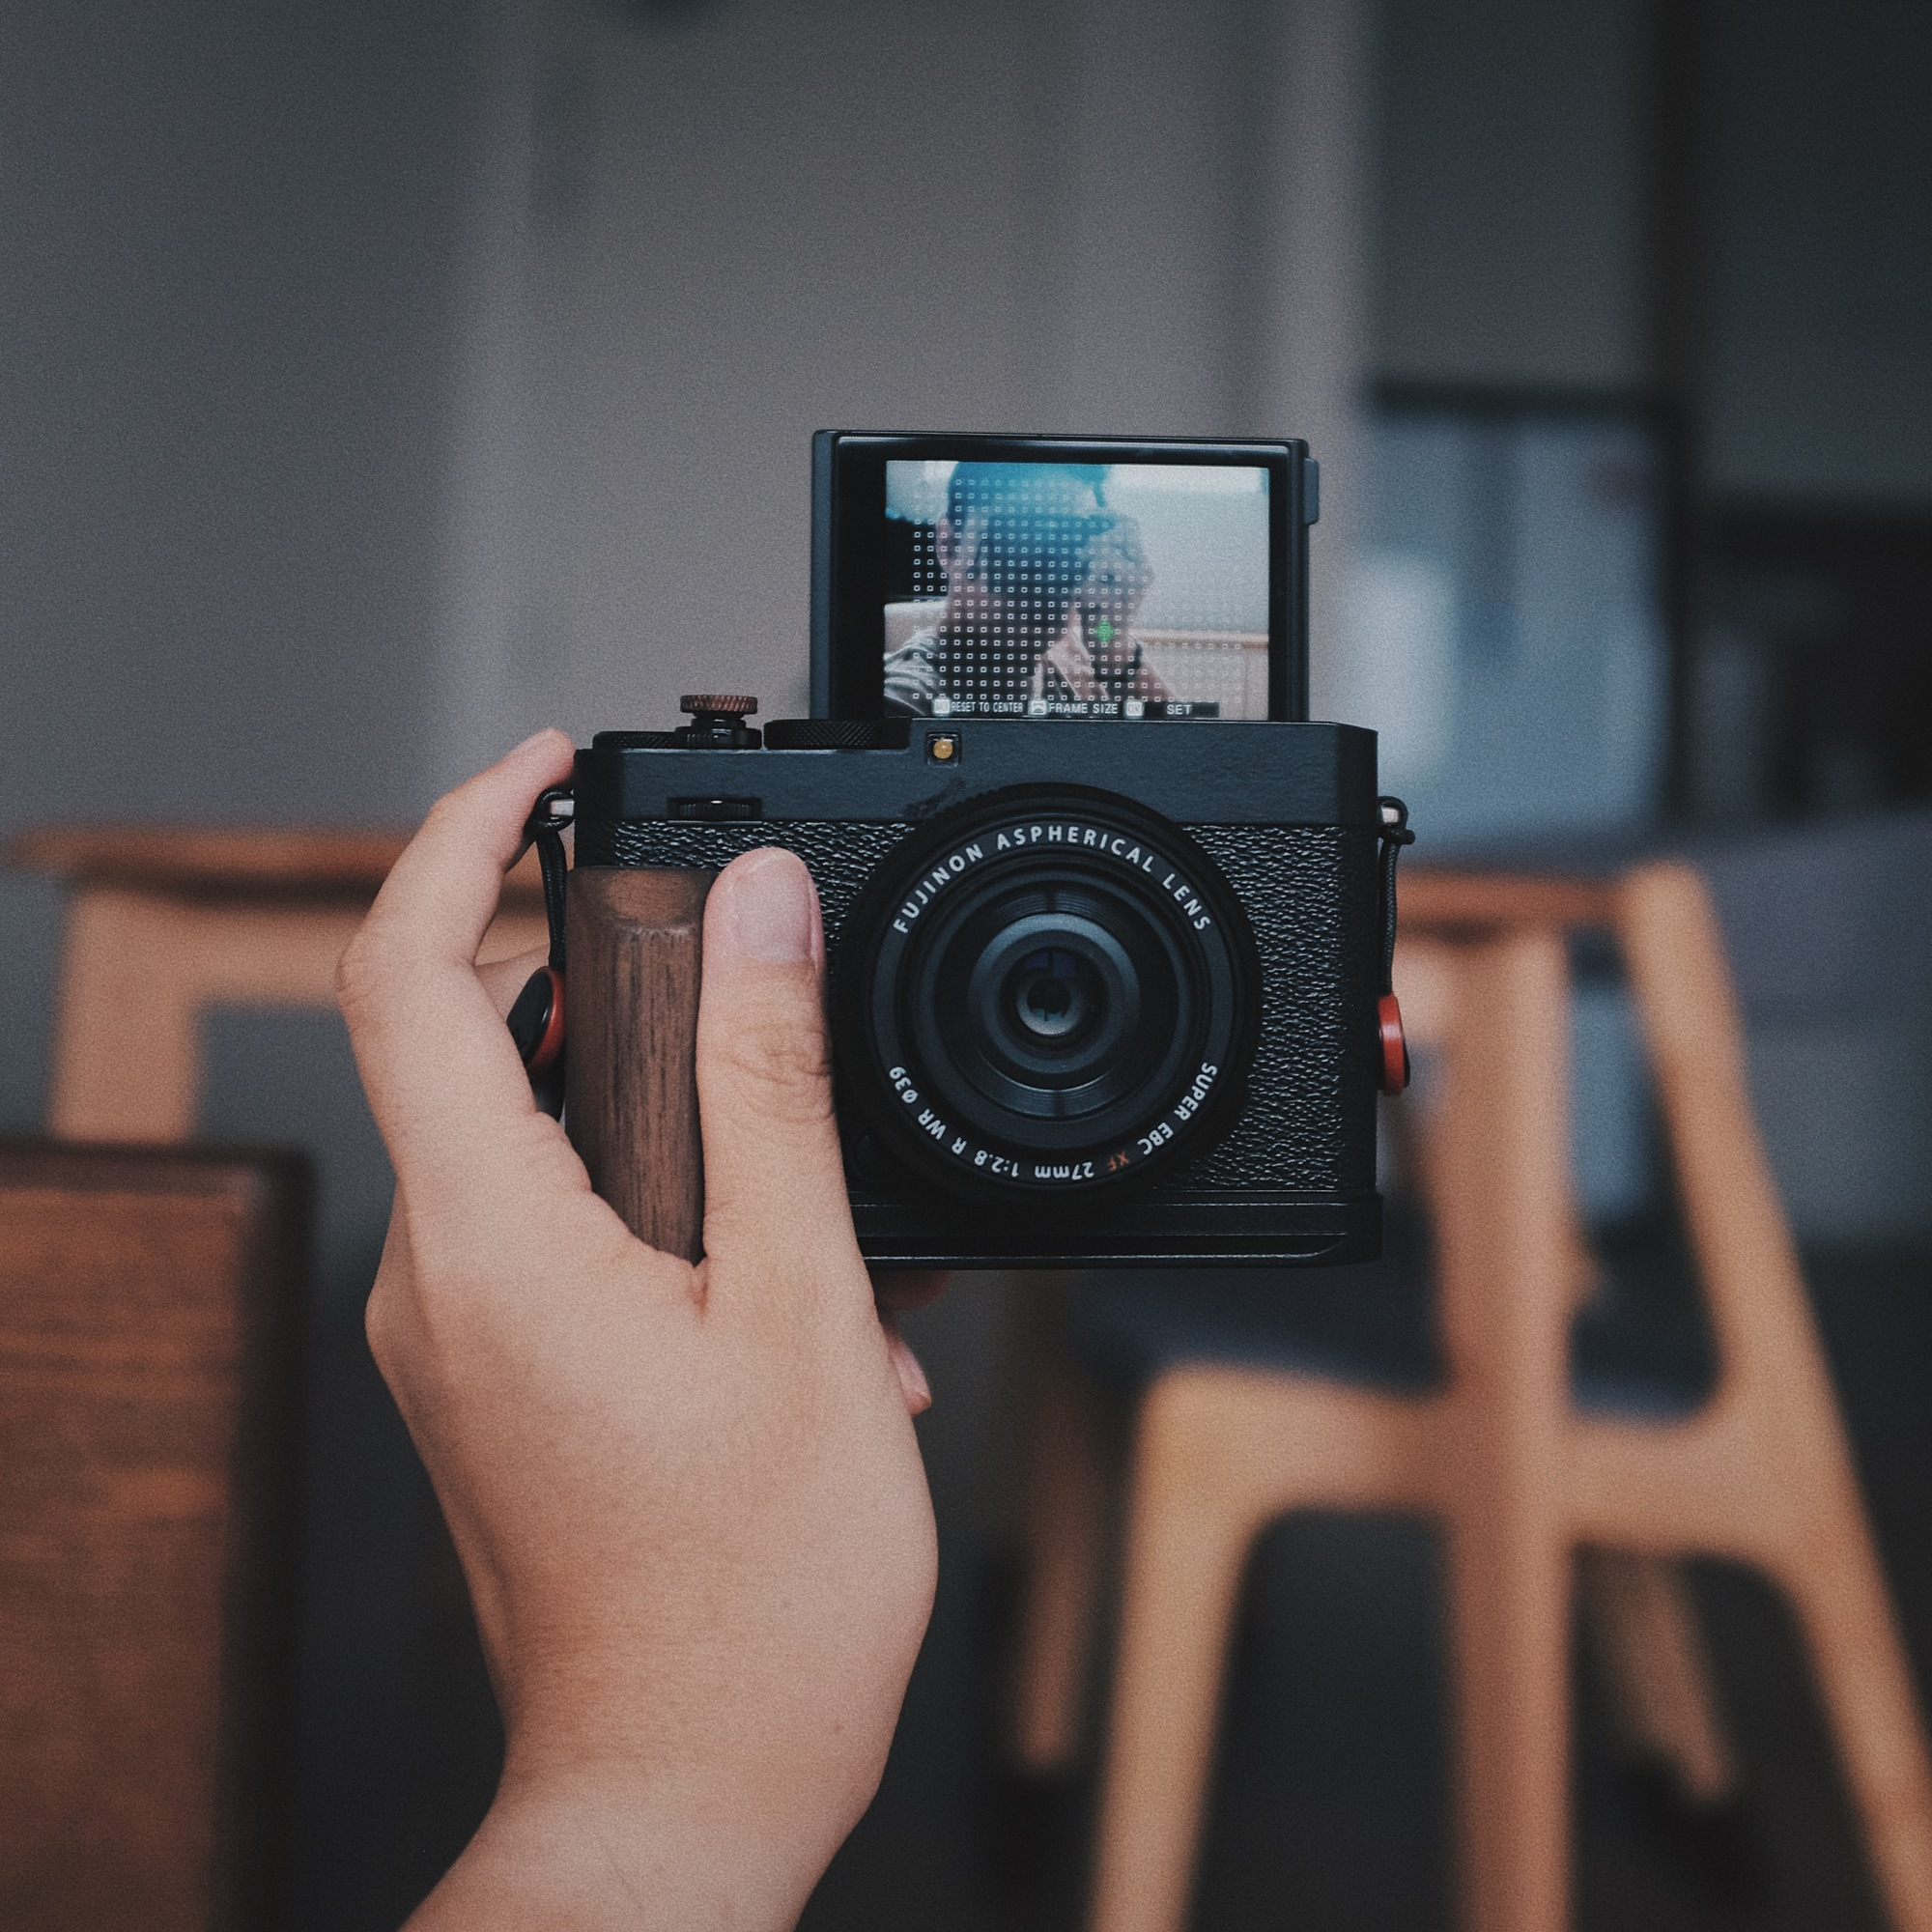
\includegraphics[width=\linewidth]{\envfinaldir/coverpic-prod.jpg}\par
            % \vskip 30pt
            \vfill

            \normalsize\rmfamily\scshape
            \copyright{} The Web Digest Project \hfill\large \envdatestr
        \end{center}
    \end{titlepage}
    % \restoregeometry
}
\newcommand{\simplehref}[1]{%
    \textcolor{blue!80!green}{\href{#1}{#1}}%
}
\renewcommand{\contentsname}{\center\Huge\sffamily\bfseries Contents\par\vskip 20pt}
\newcounter{ipartcounter}
\setcounter{ipartcounter}{0}
\newcommand{\ipart}[1]{
    % \vskip 20pt
    \clearpage
    \stepcounter{ipartcounter}
    \phantomsection
    \addcontentsline{toc}{chapter}{#1}
    % \begin{center}
    %     \Huge
    %     \sffamily\bfseries
    %     #1
    % \end{center}
    % \vskip 20pt plus 7pt
}
\newcounter{ichaptercounter}
\setcounter{ichaptercounter}{0}
\newcommand{\ichapter}[1]{
    % \vskip 20pt
    \clearpage
    \stepcounter{ichaptercounter}
    \phantomsection
    \addcontentsline{toc}{section}{\numberline{\arabic{ichaptercounter}}#1}
    \begin{center}
        \Huge
        \sffamily\bfseries
        #1
    \end{center}
    \vskip 20pt plus 7pt
}
\newcommand{\entrytitlefont}[1]{\subsection*{\raggedright\Large\sffamily\bfseries#1}}
\newcommand{\entryitemGeneric}[2]{
    % argv: title, url
    \parbox{\linewidth}{
        \entrytitlefont{#1}\par\vskip 5pt
        \footnotesize\ttfamily\mdseries
        \simplehref{#2}
    }\vskip 11pt plus 11pt minus 1pt
}
\newcommand{\entryitemGithub}[3]{
    % argv: title, url, desc
    \parbox{\linewidth}{
        \entrytitlefont{#1}\par\vskip 5pt
        \footnotesize\ttfamily\mdseries
        \simplehref{#2}\par\vskip 5pt
        \small\rmfamily\mdseries#3
    }\vskip 11pt plus 11pt minus 1pt
}
\newcommand{\entryitemAp}[3]{
    % argv: title, url, desc
    \parbox{\linewidth}{
        \entrytitlefont{#1}\par\vskip 5pt
        \footnotesize\ttfamily\mdseries
        \simplehref{#2}\par\vskip 5pt
        \small\rmfamily\mdseries#3
    }\vskip 11pt plus 11pt minus 1pt
}
\newcommand{\entryitemHackernews}[3]{
    % argv: title, hnurl, rawurl
    % \parbox{\linewidth}{
    %     \entrytitlefont{#1}\par\vskip 5pt
    %     \footnotesize\ttfamily\mdseries
    %     \simplehref{#3}\par
    %     \textcolor{black!50}{\href{#2}{#2}}
    % }\vskip 11pt plus 11pt minus 1pt
    \begin{minipage}{\linewidth}
            \entrytitlefont{#1}\par\vskip 5pt
            \footnotesize\ttfamily\mdseries
            \simplehref{#3}\par
            \textcolor{black!50}{\href{#2}{#2}}
    \end{minipage}\par\vskip 11pt plus 11pt minus 1pt
}







\begin{document}

\makeheader

\tableofcontents\clearpage




\ipart{Developers}
\ichapter{Hacker News}
\entryitemTwoLinks{US Administration announces 34\% tariffs on China – 20\% on EU}{https://news.ycombinator.com/item?id=43561253}{https://www.bbc.com/news/live/c1dr7vy39eet}

\entryitemTwoLinks{Pico.sh – SSH powered services for developers}{https://news.ycombinator.com/item?id=43560899}{https://pico.sh/}

\entryitemTwoLinks{Mozilla launching ``Thundermail'' email service to take on Gmail, Microsoft 365}{https://news.ycombinator.com/item?id=43560885}{https://www.techradar.com/pro/mozilla-launching-thundermail-email-service-to-take-on-gmail-microsoft-365}

\entryitemTwoLinks{Waltz's team set up at least 20 Signal group chats for crises across the world}{https://news.ycombinator.com/item?id=43560336}{https://www.politico.com/news/2025/04/02/waltzs-team-set-up-at-least-20-signal-group-chats-for-crises-across-the-world-00266845}

\entryitemTwoLinks{Restructuring Announcement}{https://news.ycombinator.com/item?id=43559855}{https://automattic.com/2025/04/02/restructuring-announcement/}

\entryitemTwoLinks{Tell HN: Announcing tomhow as a public moderator}{https://news.ycombinator.com/item?id=43558671}{https://news.ycombinator.com/item?id=43558671}

\entryitemTwoLinks{Matrix.org Will Migrate to MAS}{https://news.ycombinator.com/item?id=43558464}{https://matrix.org/blog/2025/04/matrix-auth-service/}

\entryitemTwoLinks{Digital Archivists: Protecting Public Data from Erasure}{https://news.ycombinator.com/item?id=43558182}{https://spectrum.ieee.org/digital-archive}

\entryitemTwoLinks{Animals Made from 13 Circles (2016)}{https://news.ycombinator.com/item?id=43557873}{https://www.dorithegiant.com/2016/05/13-animals-made-from-13-circles.html}

\entryitemTwoLinks{Porting Tailscale to Plan 9}{https://news.ycombinator.com/item?id=43557790}{https://tailscale.com/blog/plan9-port}

\entryitemTwoLinks{Nintendo unveils Switch 2 ahead of June 5 launch}{https://news.ycombinator.com/item?id=43557524}{https://arstechnica.com/gaming/2025/04/nintendo-offers-new-details-on-switch-2-hardware-software/}

\entryitemTwoLinks{Why is the world losing color?}{https://news.ycombinator.com/item?id=43557471}{https://www.culture-critic.com/p/why-is-the-world-losing-color}

\entryitemTwoLinks{How Google built its Gemini robotics models}{https://news.ycombinator.com/item?id=43557310}{https://blog.google/products/gemini/how-we-built-gemini-robotics/}

\entryitemTwoLinks{A dramatic Einstein ring seen by Webb}{https://news.ycombinator.com/item?id=43557139}{https://phys.org/news/2025-04-einstein-webb.html}

\entryitemTwoLinks{Tesla suffers worst quarter since 2022 as deliveries tumble}{https://news.ycombinator.com/item?id=43556443}{https://www.ft.com/content/0ebcec51-2a5a-4820-99e8-1e500370fd68}

\entryitemTwoLinks{Sports supplement creatine makes no difference to muscle gains, trial finds}{https://news.ycombinator.com/item?id=43556350}{https://www.unsw.edu.au/newsroom/news/2025/03/sports-supplement-creatine-makes-no-difference-to-muscle-gains-trial-finds}

\entryitemTwoLinks{A steam locomotive from 1993 broke my yarn test}{https://news.ycombinator.com/item?id=43556280}{https://blog.cloudflare.com/yarn-test-suffers-strange-derailment/}

\entryitemTwoLinks{An 'administrative error' sent a Maryland man to an El Salvador prison}{https://news.ycombinator.com/item?id=43555724}{https://apnews.com/article/el-salvador-deportation-maryland-man-trump-error-818a0fa1218de714448edcb5be1f7347}

\entryitemTwoLinks{RIP Val Kilmer: Real Genius .. the Film Nerd Culture Deserves (2015)}{https://news.ycombinator.com/item?id=43555334}{https://reactormag.com/30-years-later-real-genius-is-still-the-geek-solidarity-film-that-nerd-culture-deserves/}

\entryitemTwoLinks{Coffea stenophylla: A forgotten bean that could save coffee from extinction}{https://news.ycombinator.com/item?id=43555286}{https://www.smithsonianmag.com/science-nature/how-forgotten-bean-could-save-coffee-from-extinction-180986230/}\ichapter{Phoronix}
\entryitemGeneric{\hskip 0pt{}Linux 6.15 Further Improves AMD P-State Driver, Intel Dev Tackles A ~50\% SPEC Regression}{https://www.phoronix.com/news/Linux-6.15-ACPI-PM}

\entryitemGeneric{\hskip 0pt{}Framework Laptop 12 Pre-Orders Open Next Week}{https://www.phoronix.com/news/Framework-Laptop-12-PO}

\entryitemGeneric{\hskip 0pt{}GNOME \& KDE Plasma Wayland Sessions Outperforming Xfce + LXQt On Ubuntu 25.04 For Linux Gaming}{https://www.phoronix.com/review/ubuntu-2504-x11-gaming}

\entryitemGeneric{\hskip 0pt{}Many KVM Updates Merged For Linux 6.15}{https://www.phoronix.com/news/Linux-6.15-KVM}

\entryitemGeneric{\hskip 0pt{}Intel TDX Is Becoming Potentially Faster, Avoiding "Slow \& Buggy" Code Path On Linux}{https://www.phoronix.com/news/Intel-TDX-Avoiding-HLT-Linux}

\entryitemGeneric{\hskip 0pt{}Qt 6.9 Released With Performance Work, Better Emoji Handling \& Greater Visualizations}{https://www.phoronix.com/news/Qt-6.9-Released}

\entryitemGeneric{\hskip 0pt{}KDE Plasma 6.3.4 Now Shipping With The Latest Crash Fixes}{https://www.phoronix.com/news/KDE-Plasma-6.3.4}

\entryitemGeneric{\hskip 0pt{}Intel Linux Driver Finally Dropping The Experimental Flag For Original DG1 Graphics}{https://www.phoronix.com/news/Intel-DG1-Linux-Force-Probe}

\entryitemGeneric{\hskip 0pt{}Many Scheduler Updates In The Linux 6.15 Kernel}{https://www.phoronix.com/news/Linux-6.15-Scheduler}\ichapter{Dribbble}
\entryitemGeneric{\hskip 0pt{}Interactive Speed Slider}{https://dribbble.com/shots/25851176-Interactive-Speed-Slider}

\entryitemGeneric{\hskip 0pt{}ef monogram}{https://dribbble.com/shots/25847206-ef-monogram}

\entryitemGeneric{\hskip 0pt{}Outrigger Marketing Logo}{https://dribbble.com/shots/25848681-Outrigger-Marketing-Logo}

\entryitemGeneric{\hskip 0pt{}Letter G set}{https://dribbble.com/shots/25845864-Letter-G-set}

\entryitemGeneric{\hskip 0pt{}Helpfull - Logo Redesign}{https://dribbble.com/shots/25847828-Helpfull-Logo-Redesign}

\entryitemGeneric{\hskip 0pt{}Wayflow Logo Design - Letter W, Waves, Flow}{https://dribbble.com/shots/25847473-Wayflow-Logo-Design-Letter-W-Waves-Flow}

\entryitemGeneric{\hskip 0pt{}Vínföng Final Wordmark}{https://dribbble.com/shots/25848505-V-nf-ng-Final-Wordmark}

\entryitemGeneric{\hskip 0pt{}Prana Symbol}{https://dribbble.com/shots/25847656-Prana-Symbol}

\entryitemGeneric{\hskip 0pt{}Let down your hair}{https://dribbble.com/shots/25844844-Let-down-your-hair}

\entryitemGeneric{\hskip 0pt{}Chat GPT 4 Branding Concept}{https://dribbble.com/shots/25844194-Chat-GPT-4-Branding-Concept}

\entryitemGeneric{\hskip 0pt{}Sustainable contribution selector: percentage picker}{https://dribbble.com/shots/25843734-Sustainable-contribution-selector-percentage-picker}

\entryitemGeneric{\hskip 0pt{}FG}{https://dribbble.com/shots/25842733-FG}

\entryitemGeneric{\hskip 0pt{}Kovre Winery Logo Exploration}{https://dribbble.com/shots/25844706-Kovre-Winery-Logo-Exploration}

\entryitemGeneric{\hskip 0pt{}Cloud Paper}{https://dribbble.com/shots/25844908-Cloud-Paper}

\entryitemGeneric{\hskip 0pt{}TheStage.AI Logo Design}{https://dribbble.com/shots/25844839-TheStage-AI-Logo-Design}

\entryitemGeneric{\hskip 0pt{}Crypto Portfolio Dashboard}{https://dribbble.com/shots/25841268-Crypto-Portfolio-Dashboard}

\entryitemGeneric{\hskip 0pt{}Finergy app UI Kit on UI8}{https://dribbble.com/shots/25837473-Finergy-app-UI-Kit-on-UI8}

\entryitemGeneric{\hskip 0pt{}Weylix Logo Design - W Letter Monogram, Wave}{https://dribbble.com/shots/25834720-Weylix-Logo-Design-W-Letter-Monogram-Wave}

\entryitemGeneric{\hskip 0pt{}BB}{https://dribbble.com/shots/25834486-BB}

\entryitemGeneric{\hskip 0pt{}Fintech icons pack part 4}{https://dribbble.com/shots/25728659-Fintech-icons-pack-part-4}

\entryitemGeneric{\hskip 0pt{}Banking Mobile App Design}{https://dribbble.com/shots/25829959-Banking-Mobile-App-Design}

\entryitemGeneric{\hskip 0pt{}The Rocky token landing page}{https://dribbble.com/shots/25827682-The-Rocky-token-landing-page}

\entryitemGeneric{\hskip 0pt{}Suffo - Real Estate Landing page Animation}{https://dribbble.com/shots/25829238-Suffo-Real-Estate-Landing-page-Animation}

\entryitemGeneric{\hskip 0pt{}Mishto Logo Design}{https://dribbble.com/shots/25830165-Mishto-Logo-Design}


\ipart{Developers~~~~(zh-Hans)}
\ichapter{Solidot}
\entryitemGeneric{\hskip 0pt{}Switch 2 将于 6 月 5 日上市,起售价 450 美元}{https://www.solidot.org/story?sid=80953}

\entryitemGeneric{\hskip 0pt{}Steam 平台的 Linux 份额达到 2.33\%}{https://www.solidot.org/story?sid=80952}

\entryitemGeneric{\hskip 0pt{}到本世纪末如果全球气温上升 3°C 全世界四成经济可能会被抹掉}{https://www.solidot.org/story?sid=80951}

\entryitemGeneric{\hskip 0pt{}年轻男性泡冷水澡或有助于身体健康}{https://www.solidot.org/story?sid=80950}

\entryitemGeneric{\hskip 0pt{}每周三天间歇性禁食减肥效果显著}{https://www.solidot.org/story?sid=80949}

\entryitemGeneric{\hskip 0pt{}OpenAI 被指控未经授权使用 O'Reilly 书籍训练 GPT-4o}{https://www.solidot.org/story?sid=80948}

\entryitemGeneric{\hskip 0pt{}Mozilla 准备推出付费版 Thunderbird Pro}{https://www.solidot.org/story?sid=80947}

\entryitemGeneric{\hskip 0pt{}小米 SU7 发生涉及智驾的致命车祸}{https://www.solidot.org/story?sid=80946}

\entryitemGeneric{\hskip 0pt{}互联网如何影响现实生活}{https://www.solidot.org/story?sid=80945}

\entryitemGeneric{\hskip 0pt{}为维持竞争优势 DeepMind 推迟发布 AI 研究论文}{https://www.solidot.org/story?sid=80944}

\entryitemGeneric{\hskip 0pt{}期刊尝试给审稿人付费}{https://www.solidot.org/story?sid=80943}

\entryitemGeneric{\hskip 0pt{}睡前看屏幕增加失眠风险}{https://www.solidot.org/story?sid=80942}

\entryitemGeneric{\hskip 0pt{}Pidgin 3.0.0 Experimental 2 释出}{https://www.solidot.org/story?sid=80941}

\entryitemGeneric{\hskip 0pt{}Mozilla 释出 Firefox 137}{https://www.solidot.org/story?sid=80940}

\entryitemGeneric{\hskip 0pt{}Google 向免费用户提供 Gemini 2.5 Pro (Experimental) }{https://www.solidot.org/story?sid=80939}

\entryitemGeneric{\hskip 0pt{}韩国游戏工作室竞争开发星际争霸新作}{https://www.solidot.org/story?sid=80938}

\entryitemGeneric{\hskip 0pt{}英特尔 CEO 陈立武表示将剥离非核心部门}{https://www.solidot.org/story?sid=80936}

\entryitemGeneric{\hskip 0pt{}Netflix CEO 称电影院正在死亡}{https://www.solidot.org/story?sid=80935}

\entryitemGeneric{\hskip 0pt{}微软关闭了位于上海的物联网和 AI 实验室}{https://www.solidot.org/story?sid=80934}

\entryitemGeneric{\hskip 0pt{}白领工人的工作可能开始减少}{https://www.solidot.org/story?sid=80933}\ichapter{V2EX}
\entryitemGeneric{\hskip 0pt{}[云修电脑] 大佬们,求助。台式机电脑主板 bios 红灯常量,显示器无信号}{https://www.v2ex.com/t/1122991}

\entryitemGeneric{\hskip 0pt{}[Apple] Infuse 更新,支持 115 网盘和百度网盘了}{https://www.v2ex.com/t/1122990}

\entryitemGeneric{\hskip 0pt{}[日本] 想要请教一下像新加坡这样的护照可以在日本买房吗?就是旅游性质的}{https://www.v2ex.com/t/1122989}

\entryitemGeneric{\hskip 0pt{}[OpenAI] ChatGPT 新版画图不限次数, V2EX 用户免费送}{https://www.v2ex.com/t/1122987}

\entryitemGeneric{\hskip 0pt{}[程序员] Jenkins 的 SSH Pipeline Steps 插件的 sshPut 功能在传输单个文件时如何不复制本地目录结构?}{https://www.v2ex.com/t/1122986}

\entryitemGeneric{\hskip 0pt{}[WordPress] 求推荐类似 B2 的主题,但是是国外版本的,最好带有商城,社区及发布文章这些的?}{https://www.v2ex.com/t/1122985}

\entryitemGeneric{\hskip 0pt{}[问与答] 老哥们 Windows 用 Clash Verge 如何使用自己的机场订阅并使用别人的策略组呢?}{https://www.v2ex.com/t/1122983}

\entryitemGeneric{\hskip 0pt{}[创业组队] 有没有会安卓/IOS 开发的朋友,最近有空一起搞一个 AI 项目分钱}{https://www.v2ex.com/t/1122982}

\entryitemGeneric{\hskip 0pt{}[分享创造] 分享自用的音乐 App,集成 QQ 音乐/网易云音乐/喜马拉雅,目前仅支持安卓}{https://www.v2ex.com/t/1122981}

\entryitemGeneric{\hskip 0pt{}[分享创造] 下班用 ai 搓了个网站,大家帮忙看看}{https://www.v2ex.com/t/1122979}

\entryitemGeneric{\hskip 0pt{}[云计算] 请问哪个对象存储供应商对内地友好又能全球同步的}{https://www.v2ex.com/t/1122978}

\entryitemGeneric{\hskip 0pt{}[汽车] 忍不住要买 14.9 万的比亚迪汉 ev605 了,请问有什么缺点吗?}{https://www.v2ex.com/t/1122976}

\entryitemGeneric{\hskip 0pt{}[问与答] 是否有网站上有把英伟达,华为昇腾,海光之类的 GPU 对比的列表?找了很久都没有找到呢。}{https://www.v2ex.com/t/1122974}

\entryitemGeneric{\hskip 0pt{}[问与答] 没想到 pdd 的 app 大小居然在 80 来 M 左右的大小}{https://www.v2ex.com/t/1122973}

\entryitemGeneric{\hskip 0pt{}[问与答] 求推荐国内本地测速平台}{https://www.v2ex.com/t/1122971}

\entryitemGeneric{\hskip 0pt{}[Adobe] PS logo 设计+ 封面设计,有偿}{https://www.v2ex.com/t/1122970}

\entryitemGeneric{\hskip 0pt{}[Nintendo Switch] 你对新发布的 Switch2 感冒嘛?}{https://www.v2ex.com/t/1122969}

\entryitemGeneric{\hskip 0pt{}[macOS] 微信 4.0 mac 版是不是打开图片有延迟}{https://www.v2ex.com/t/1122968}

\entryitemGeneric{\hskip 0pt{}[VPS] 求推荐日本 VPS}{https://www.v2ex.com/t/1122967}

\entryitemGeneric{\hskip 0pt{}[问与答] autojs 无法分析一个 app 的界面}{https://www.v2ex.com/t/1122966}

\entryitemGeneric{\hskip 0pt{}[分享创造] 一个猛男粉设计的鼠标手势扩展}{https://www.v2ex.com/t/1122964}

\entryitemGeneric{\hskip 0pt{}[分享创造] 一个小程序帮你发现日常生活中的诗意}{https://www.v2ex.com/t/1122963}

\entryitemGeneric{\hskip 0pt{}[VPS] 有适合用来搭游戏服务器的 vps 推荐吗?}{https://www.v2ex.com/t/1122962}

\entryitemGeneric{\hskip 0pt{}[程序员] 找一个开源的通用用户管理系统}{https://www.v2ex.com/t/1122961}

\entryitemGeneric{\hskip 0pt{}[macOS] MacOS 移除私有化接口,需要的谨慎升级。}{https://www.v2ex.com/t/1122960}

\entryitemGeneric{\hskip 0pt{}[问与答] 阿里云国际想开个号登上去就反诈}{https://www.v2ex.com/t/1122959}

\entryitemGeneric{\hskip 0pt{}[生活] 大家有没有觉得周围人近几年肤色明显变深?}{https://www.v2ex.com/t/1122958}

\entryitemGeneric{\hskip 0pt{}[分享创造] 给 Thorium 浏览器写了个用来升级的工具 被作者留意到了}{https://www.v2ex.com/t/1122957}

\entryitemGeneric{\hskip 0pt{}[问与答] 不懂就问:大家笔记本的系统硬盘有坏过吗}{https://www.v2ex.com/t/1122956}

\entryitemGeneric{\hskip 0pt{}[问与答] 微信小程序中已发货但未结算部分的钱会体现在商户号余额中吗?}{https://www.v2ex.com/t/1122955}

\entryitemGeneric{\hskip 0pt{}[汽车] 为什么现在的汽车都要带天窗,甚至是全景天幕?}{https://www.v2ex.com/t/1122954}

\entryitemGeneric{\hskip 0pt{}[问与答] 求大佬推荐个 window 清理垃圾的软件, C 盘莫名其妙多了不少}{https://www.v2ex.com/t/1122952}

\entryitemGeneric{\hskip 0pt{}[业界八卦] 请教:这个网站看着挺漂亮的,用的什么前端技术、UI 框架?}{https://www.v2ex.com/t/1122951}

\entryitemGeneric{\hskip 0pt{}[宽带症候群] 家里的联通宽带莫名其妙有了公网 ip 疑惑??}{https://www.v2ex.com/t/1122950}

\entryitemGeneric{\hskip 0pt{}[Tesla] 有必要 ota 更新车机的系统吗}{https://www.v2ex.com/t/1122949}

\entryitemGeneric{\hskip 0pt{}[宽带症候群] TailScale 组网时 IPv6 遇到 UDP QOS ,有无朋友有类似情况或者解决办法?}{https://www.v2ex.com/t/1122948}

\entryitemGeneric{\hskip 0pt{}[生活] 问问大家用的什么铁锅?要换锅}{https://www.v2ex.com/t/1122947}

\entryitemGeneric{\hskip 0pt{}[NAS] 有没有占内存小、内网用、开源的 stmp 服务}{https://www.v2ex.com/t/1122946}

\entryitemGeneric{\hskip 0pt{}[职场话题] 被领导谈话劝退了,工作之于的特别惊喜}{https://www.v2ex.com/t/1122945}

\entryitemGeneric{\hskip 0pt{}[问与答] 请教一下, 2025 年软路由、旁路由最佳方案是什么}{https://www.v2ex.com/t/1122944}

\entryitemGeneric{\hskip 0pt{}[Bitcoin] [广州/后端开发] 国内领先的 Web3 AI 公司,前景好,高成长性}{https://www.v2ex.com/t/1122943}

\entryitemGeneric{\hskip 0pt{}[分享创造] https://hf-mirror.com/的 hfd.sh 调用 Windows 中的迅雷,加速模型和数据集下载}{https://www.v2ex.com/t/1122942}

\entryitemGeneric{\hskip 0pt{}[程序员] 类似 bugly.qq.com 这样用于上报或监控的域名有哪些?有整理的项目吗?是否可以直接屏蔽?}{https://www.v2ex.com/t/1122941}

\entryitemGeneric{\hskip 0pt{}[Apple] 一个关于 iPhone 相机按钮为什么会是现在这个半成品样子的猜想}{https://www.v2ex.com/t/1122938}

\entryitemGeneric{\hskip 0pt{}[电动汽车] 小米事件发生后,我建议科比起诉直升机厂家}{https://www.v2ex.com/t/1122937}

\entryitemGeneric{\hskip 0pt{}[电动汽车] 同样发生车祸、事故,为何燃油车比电车少争议?}{https://www.v2ex.com/t/1122935}

\entryitemGeneric{\hskip 0pt{}[分享创造] 全键盘手机爱好者的福音,复刻黑莓 Q20, Key1}{https://www.v2ex.com/t/1122934}

\entryitemGeneric{\hskip 0pt{}[NAS] 群晖硬盘 SMART 检测结果为``需要注意'',是不是硬盘要挂了啊}{https://www.v2ex.com/t/1122933}

\entryitemGeneric{\hskip 0pt{}[分享发现] 发现一个模拟器游戏镜像的收藏, 15T+}{https://www.v2ex.com/t/1122931}

\entryitemGeneric{\hskip 0pt{}[酷工作] 深圳寻求 Python 开发工程师}{https://www.v2ex.com/t/1122930}


\ipart{Generic News}







\clearpage
\leavevmode\vfill
\footnotesize

Copyright \copyright{} 2023-2025 Neruthes and other contributors.

This document is published with CC BY-NC-ND 4.0 license.

The entries listed in this newsletter may be copyrighted by their respective creators.

This newsletter is generated by the Web Digest project.

The newsletters are also delivered via Telegram channel \CJKunderline{\href{https://t.me/webdigestchannel}{https://t.me/webdigestchannel}}.\\
RSS feed is available at \CJKunderline{\href{https://webdigest.pages.dev/rss.xml}{https://webdigest.pages.dev/rss.xml}}.

This newsletter is available in PDF at
\CJKunderline{\href{https://webdigest.pages.dev/}{https://webdigest.pages.dev/}}.

The source code being used to generate this newsletter is available at\\
\CJKunderline{\href{https://github.com/neruthes/webdigest}{https://github.com/neruthes/webdigest}}.

This newsletter is also available in
\CJKunderline{\href{http://webdigest.pages.dev/readhtml/\envyear/WebDigest-20250403.html}{HTML}} and
\CJKunderline{\href{https://github.com/neruthes/webdigest/blob/master/markdown/\envyear/WebDigest-20250403.md}{Markdown}}.


\coverpic{https://unsplash.com/photos/steamed-buns-in-a-bamboo-steamer-c3U4xmOSWc8}{Mathias Reding}


\end{document}
